\begin{figure}
    \usetikzlibrary{positioning, shapes.arrows, shapes.geometric, fit, calc, backgrounds}

    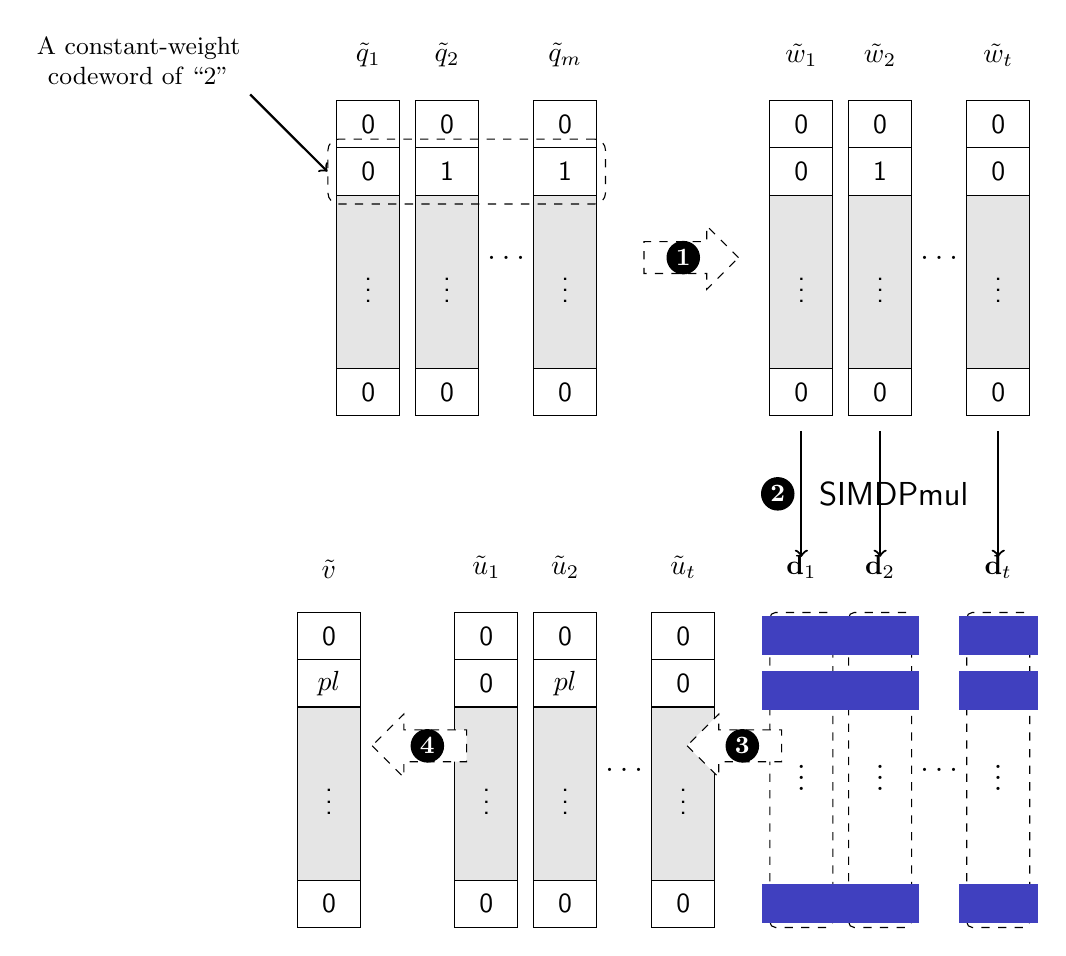
\begin{tikzpicture}[
        font=\sffamily,
        node distance=0.5cm,
        cell/.style={draw, minimum width=0.8cm, minimum height=0.6cm, inner sep=0pt, anchor=north, fill=white},
        graybar/.style={draw, fill=gray!20, minimum width=0.8cm, minimum height=2.2cm, anchor=north},
        bluebar/.style={fill=blue!50!gray, minimum width=1.0cm, minimum height=0.5cm},
        dashedcol/.style={draw, dashed, rounded corners=2pt, minimum width=0.8cm, minimum height=4.0cm, anchor=north},
        labeltext/.style={anchor=south, yshift=1mm},
        stepcircle/.style={circle, fill=black, text=white, font=\bfseries\small, inner sep=1.5pt},
        blockarrow/.style={single arrow, draw, dashed, fill=white, minimum height=1.2cm, single arrow head extend=0.2cm, shape border rotate=#1},
        dotstyle/.style={font=\large}
    ]

    % --- Group Q (Top Left) ---
    % Coordinates relative to (0,0)

    % Column q1
    \node[labeltext] at (0, 0.2) {$\tilde{q}_1$};
    \node[cell] (q1_1) at (0, 0) {0};
    \node[cell] (q1_2) at (0, -0.6) {0};
    \node[graybar] (q1_mid) at (0, -1.2) {$\vdots$};
    \node[cell] (q1_3) at (0, -3.4) {0};

    % Column q2
    \node[labeltext] at (1, 0.2) {$\tilde{q}_2$};
    \node[cell] (q2_1) at (1, 0) {0};
    \node[cell] (q2_2) at (1, -0.6) {1};
    \node[graybar] (q2_mid) at (1, -1.2) {$\vdots$};
    \node[cell] (q2_3) at (1, -3.4) {0};

    % Dots between q2 and qm
    \node[dotstyle] at (1.75, -2) {$\dots$};

    % Column qm
    \node[labeltext] at (2.5, 0.2) {$\tilde{q}_m$};
    \node[cell] (qm_1) at (2.5, 0) {0};
    \node[cell] (qm_2) at (2.5, -0.6) {1};
    \node[graybar] (qm_mid) at (2.5, -1.2) {$\vdots$};
    \node[cell] (qm_3) at (2.5, -3.4) {0};

    % Highlight box for row 2
    \node[draw, dashed, rounded corners, inner sep=3pt, fit=(q1_2) (qm_2)] (highlight) {};

    % Annotation for highlight
    \node[anchor=east, align=center, font=\small] (note) at (-1.5, 0.5) {A constant-weight\\codeword of ``2''};
    \draw[->, thick] (note.south east) -- (highlight.west);


    % --- Group W (Top Right) ---
    % Shifted right

    % Column w1
    \begin{scope}[xshift=5.5cm]
    \node[labeltext] at (0, 0.2) {$\tilde{w}_1$};
    \node[cell] (w1_1) at (0, 0) {0};
    \node[cell] (w1_2) at (0, -0.6) {0};
    \node[graybar] (w1_mid) at (0, -1.2) {$\vdots$};
    \node[cell] (w1_3) at (0, -3.4) {0};

    % Column w2
    \node[labeltext] at (1, 0.2) {$\tilde{w}_2$};
    \node[cell] (w2_1) at (1, 0) {0};
    \node[cell] (w2_2) at (1, -0.6) {1};
    \node[graybar] (w2_mid) at (1, -1.2) {$\vdots$};
    \node[cell] (w2_3) at (1, -3.4) {0};

    % Dots
    \node[dotstyle] at (1.75, -2) {$\dots$};

    % Column wt
    \node[labeltext] at (2.5, 0.2) {$\tilde{w}_t$};
    \node[cell] (wt_1) at (2.5, 0) {0};
    \node[cell] (wt_2) at (2.5, -0.6) {0};
    \node[graybar] (wt_mid) at (2.5, -1.2) {$\vdots$};
    \node[cell] (wt_3) at (2.5, -3.4) {0};
    \end{scope}

    % Arrow 1 (Between Q and W)
    \node[blockarrow=0, anchor=center] at (4.0, -2) {\phantom{xx}};
    \node[stepcircle] at (4.0, -2) {1};


    % --- Group D (Bottom Right) ---
    % Below W

    \begin{scope}[xshift=5.5cm, yshift=-6.5cm]
    % Column d1
    \node[labeltext] at (0, 0.2) {$\mathbf{d}_1$};
    \node[dashedcol] (d1_outline) at (0, 0) {};
    \node[bluebar] at (0, -0.3) {};
    \node[bluebar] at (0, -1.0) {};
    \node[font=\large] at (0, -2.0) {$\vdots$};
    \node[bluebar] at (0, -3.7) {};

    % Column d2
    \node[labeltext] at (1, 0.2) {$\mathbf{d}_2$};
    \node[dashedcol] (d2_outline) at (1, 0) {};
    \node[bluebar] at (1, -0.3) {};
    \node[bluebar] at (1, -1.0) {};
    \node[font=\large] at (1, -2.0) {$\vdots$};
    \node[bluebar] at (1, -3.7) {};

    % Dots
    \node[dotstyle] at (1.75, -2) {$\dots$};

    % Column dt
    \node[labeltext] at (2.5, 0.2) {$\mathbf{d}_t$};
    \node[dashedcol] (dt_outline) at (2.5, 0) {};
    \node[bluebar] at (2.5, -0.3) {};
    \node[bluebar] at (2.5, -1.0) {};
    \node[font=\large] at (2.5, -2.0) {$\vdots$};
    \node[bluebar] at (2.5, -3.7) {};
    \end{scope}

    % Arrow 2 (From W to D)
    % Arrows
    \draw[->, thick] (5.5, -4.2) -- (5.5, -5.8);
    \draw[->, thick] (6.5, -4.2) -- (6.5, -5.8);
    \draw[->, thick] (8.0, -4.2) -- (8.0, -5.8);

    % Label and Circle
    \node[stepcircle] at (5.2, -5.0) {2};
    \node[anchor=west, font=\sffamily\large] at (5.6, -5.0) {SIMDPmul};


    % --- Group U (Bottom Middle) ---
    % Left of D

    \begin{scope}[xshift=1.5cm, yshift=-6.5cm]
    % Column u1
    \node[labeltext] at (0, 0.2) {$\tilde{u}_1$};
    \node[cell] (u1_1) at (0, 0) {0};
    \node[cell] (u1_2) at (0, -0.6) {0};
    \node[graybar] (u1_mid) at (0, -1.2) {$\vdots$};
    \node[cell] (u1_3) at (0, -3.4) {0};

    % Column u2
    \node[labeltext] at (1, 0.2) {$\tilde{u}_2$};
    \node[cell] (u2_1) at (1, 0) {0};
    \node[cell] (u2_2) at (1, -0.6) {$pl$};
    \node[graybar] (u2_mid) at (1, -1.2) {$\vdots$};
    \node[cell] (u2_3) at (1, -3.4) {0};

    % Dots
    \node[dotstyle] at (1.75, -2) {$\dots$};

    % Column ut
    \node[labeltext] at (2.5, 0.2) {$\tilde{u}_t$};
    \node[cell] (ut_1) at (2.5, 0) {0};
    \node[cell] (ut_2) at (2.5, -0.6) {0};
    \node[graybar] (ut_mid) at (2.5, -1.2) {$\vdots$};
    \node[cell] (ut_3) at (2.5, -3.4) {0};
    \end{scope}

    % Arrow 3 (From D to U)
    \node[blockarrow=180, anchor=center] at (4.75, -8.2) {\phantom{xx}};
    \node[stepcircle] at (4.75, -8.2) {3};


    % --- Group V (Bottom Left) ---
    % Left of U

    \begin{scope}[xshift=-0.5cm, yshift=-6.5cm]
    % Column v
    \node[labeltext] at (0, 0.2) {$\tilde{v}$};
    \node[cell] (v_1) at (0, 0) {0};
    \node[cell] (v_2) at (0, -0.6) {$pl$};
    \node[graybar] (v_mid) at (0, -1.2) {$\vdots$};
    \node[cell] (v_3) at (0, -3.4) {0};
    \end{scope}

    % Arrow 4 (From U to V)
    \node[blockarrow=180, anchor=center] at (0.75, -8.2) {\phantom{xx}};
    \node[stepcircle] at (0.75, -8.2) {4};

    \end{tikzpicture}
\end{figure}